
%(BEGIN_QUESTION)
% Copyright 2013, Tony R. Kuphaldt, released under the Creative Commons Attribution License (v 1.0)
% This means you may do almost anything with this work of mine, so long as you give me proper credit

In this process, maple syrup is heated through a series of heat exchangers, then enters an evaporator vessel where the water boils off into vapor.  The purpose of this is to raise the sugar concentration of the syrup, making it suitable for use as a food topping.  Several temperature gauges (TG) monitor the temperatures of different fluids in the process:

$$\includegraphics[width=15.5cm]{i02548x01.eps}$$

Identify which temperature gauge in each pair should register a {\it higher} temperature:

\begin{itemize}
\item{} TG-49 or TG-54?
\vskip 5pt
\item{} TG-41 or TG-84
\vskip 5pt
\item{} TG-49 or TG-75?
\vskip 5pt
\item{} TG-41 or TG-75?
\vskip 5pt
\item{} TG-52 or TG-54?
\end{itemize}

\underbar{file i02548}
%(END_QUESTION)





%(BEGIN_ANSWER)

\begin{itemize}
\item{} {\bf TG-49} is hotter than TG-54
\item{} {\bf TG-41} is hotter than TG-84
\item{} {\bf TG-49} is hotter than TG-75
\item{} {\bf TG-41} is hotter than TG-75
\item{} TG-52 is colder than {\bf TG-54}
\end{itemize}


%(END_ANSWER)





%(BEGIN_NOTES)


%INDEX% Process: maple syrup concentration (single-effect evaporator)

%(END_NOTES)


